\subsection{Impact of neural network depth on validation accuracy}
\label{subsection:experiments:classification:depth}
In this subsection, we will discuss the relationship between the best validation accuracy and neural network depth. The experiment setup and methodology are almost identical to the previous subsection. The only change is the addition of multiple identical hidden layers instead of a single hidden layer.
In the previous subsection, we observed that the addition of a single identical layer did not significantly improve the validation accuracy. According to the results presented in Figure \ref{figure:experiments:classification:depth:64} and in Figure \ref{figure:experiments:classification:depth:128}, validation accuracy does not improve with addition of identically wide hidden layers. Hence, we may conjecture that on this dataset, deeper fully-connected networks do not generalize better than shallow fully-connected networks. It is important to note that results are consistent across all activation functions. 
Moreover, results in Figure \ref{figure:experiments:classification:depth:64} and Figure \ref{figure:experiments:classification:depth:128} are almost identical. This can be attributed to the apparent similarity in neural network architecture.

It is interesting to note that the validation accuracy remains close to $80 \%$ for networks with at most 4 layers. However, as the number of layers increases, the validation accuracy significantly decreases. This observation applies to all activation functions. However the validation accuracy drop is the largest for $\operatorname{sigmoid}$ and $\tanh$. This can be attributed to a well-known \textit{vanishing gradient} problem. We will briefly discuss that source of difficulty in training deep neural networks with $\operatorname{sigmoid}$ activation. We know that $\lim_{x \to \infty} \sigma (x) = 1$ and $\lim_{x \to -\infty} \sigma (x) = 0$. By Lemma \ref{lemma:introduction:activation:sigmoid-derivative}, we conclude that $\lim_{x \to \infty} \sigma'(x) = 0$ and $\lim_{x \to -\infty} \sigma'(x) = 0$. Informally, as the inputs of a $\operatorname{sigmoid}$ layer become extremely small or extremely large, the gradient of the loss function with respect to parameters of a $\operatorname{sigmoid}$ layer vanishes. This causes serious problems in gradient-based optimization since the corresponding weights and biases cease to update. However, in case of $\operatorname{ReLU}$, the drop in validation accuracy resulting from increased depth is noticeably smaller than in case of $\operatorname{sigmoid}$ and $\tanh$. This is also a known result and one of key reasons why $\operatorname{ReLU}$ is preferred to $\operatorname{sigmoid}$ and $\tanh$ when training deep networks.

\begin{figure}[H]
    \centering
    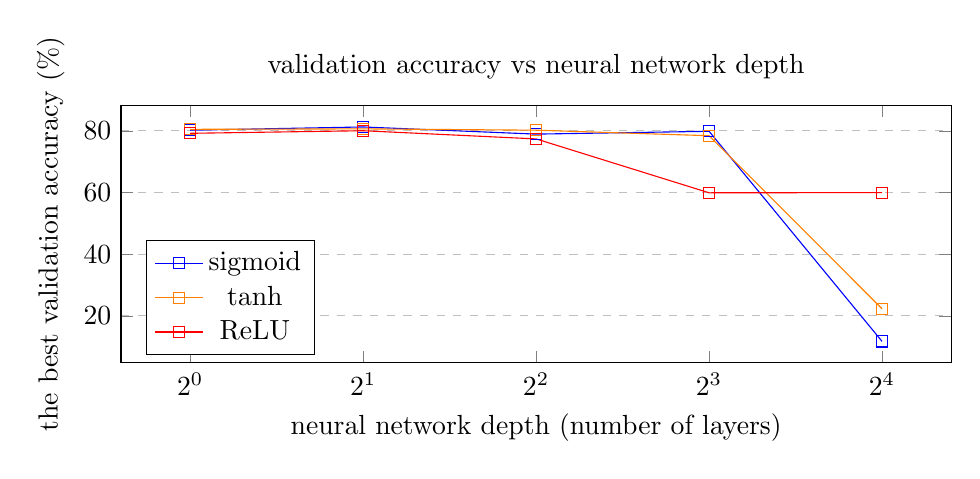
\begin{tikzpicture}
        \begin{axis}[
            height=0.4\textwidth,
            width=\textwidth,
            title= {validation accuracy vs neural network depth},
            xlabel={neural network depth (number of layers)},
            ylabel={the best validation accuracy (\%)},
            ymajorgrids=true,
            grid style=dashed,
            xmode=log,
            legend pos=south west,
            log basis x={2}]
            \addplot[mark=square,blue] coordinates {(1,80.24) (2,81.29) (4, 78.97) (8,79.88) (16,11.72)};
            \addplot[mark=square,orange] coordinates {(1,80.52) (2,80.67) (4,80.24) (8,78.45) (16,22.30)};
            \addplot[mark=square,red] coordinates {(1,79.23) (2,80.07) (4,77.41) (8,59.93) (16,60.00)};
            \legend{sigmoid, tanh, ReLU}
        \end{axis}
    \end{tikzpicture}
    \caption{Effects of varying neural network depth while keeping layer width of \textbf{64 neurons}}
    \label{figure:experiments:classification:depth:64}
\end{figure}
\begin{figure}[H]
    \centering
    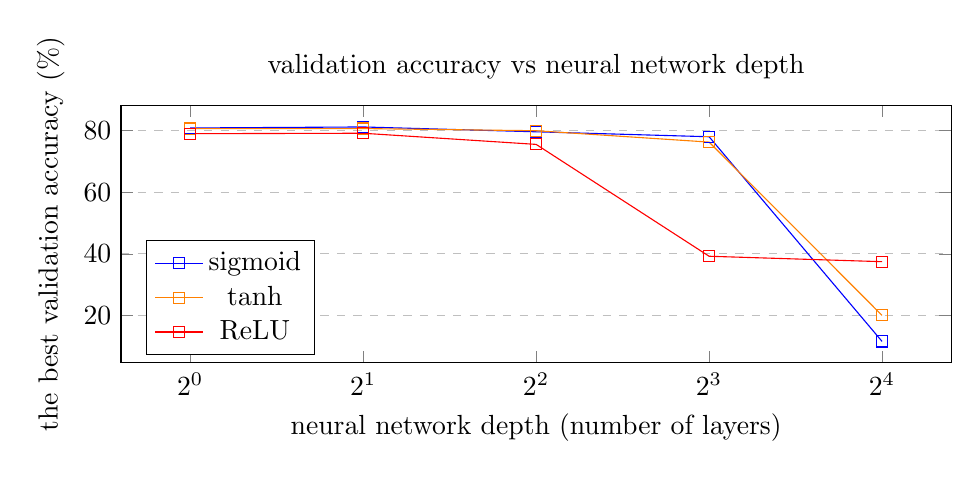
\begin{tikzpicture}
        \begin{axis}[
            height=0.4\textwidth,
            width=\textwidth,
            title= {validation accuracy vs neural network depth},
            xlabel={neural network depth (number of layers)},
            ylabel={the best validation accuracy  (\%)},
            ymajorgrids=true,
            grid style=dashed,
            xmode=log,
            legend pos=south west,
            log basis x={2}]
            \addplot[mark=square,blue] coordinates {(1,80.82) (2,81.15) (4, 79.58) (8,77.98) (16,11.60)};
            \addplot[mark=square,orange] coordinates {(1,80.63) (2,80.63) (4,79.93) (8,76.24) (16,20.05)};
            \addplot[mark=square,red] coordinates {(1,78.97) (2,79.11) (4,75.50) (8,39.22) (16,37.46)};
            \legend{sigmoid, tanh, ReLU}
        \end{axis}
    \end{tikzpicture}
    \caption{Effects of varying neural network depth while keeping layer width of \textbf{128 neurons}}
    \label{figure:experiments:classification:depth:128}
\end{figure}